\documentclass{article}
\usepackage[margin=1in]{geometry}
\usepackage{mathtools, amsfonts, amsthm, graphicx, listings, xcolor, pdfpages}


\definecolor{codegreen}{rgb}{0,0.6,0}
\definecolor{codegray}{rgb}{0.5,0.5,0.5}
\definecolor{codepurple}{rgb}{0.58,0,0.82}
\definecolor{backcolour}{rgb}{0.95,0.95,0.92}

\lstdefinestyle{mystyle}{
    backgroundcolor=\color{backcolour},   
    commentstyle=\color{codegreen},
    keywordstyle=\color{magenta},
    numberstyle=\tiny\color{codegray},
    stringstyle=\color{codepurple},
    basicstyle=\ttfamily\footnotesize,
    breakatwhitespace=false,         
    breaklines=true,                 
    captionpos=b,                    
    keepspaces=true,                 
    numbers=left,                    
    numbersep=5pt,                  
    showspaces=false,                
    showstringspaces=false,
    showtabs=false,                  
    tabsize=2
}

\lstset{style=mystyle}

\title{HW06}
\author{Sam Ly}

\begin{document}
\maketitle

\section*{Required Exercise 1 [4]}

Done.

\section*{Required Exercise 2 [3]}

Let \(F_1 = F_2 = 1\), and \(F_n = F_{n-1} + F_{n-1}\) for \(n \ge 3\). Use 
induction to prove that \(F_n\) is even if and only if \(3 \mid n\).

\begin{proof}
    First, we must see that the sum of two integers \(a\) and \(b\) is even if 
    and only if \(a\) and \(b \) have the same parity. In other words, if \(a\) 
    and \(b\) are both even or odd, then \(a + b\) is even. But if \(a\) is even 
    and \(b\) is odd or vice versa, then \(a + b \) is odd. 

    We can procede with induction. We use the following as our base cases: 
    \begin{enumerate}
        \item \(F_1 = 1\)
        \item \(F_2 = 1\)
        \item \(F_3 = 1\)
    \end{enumerate}

    Then, we assume that \(F_n\) is even if and only if \(3 \mid n\) for all 
    \(n \le k\), where \(3 \mid k\).

    Thus, \(F_k\) is even, and \(F_{k-1}\) and \(F_{k-2}\) are both odd. 

    Then, we see that \(F_{k+1}\) must be odd, since \(F_{k+1} = F_k + F_{k-1}\) 
    and \(F_k\) is even while \(F_{k-1}\) is odd. 

    Similarly, we see that \(F_{k+2}\) must also be odd, since \(F_{k+1}\) is odd 
    and \(F_k\) is even. 

    We also notice that \(k+1\) and \(k+2\) must not be divisible by 3 because
    \begin{align*}
        k &\equiv 0 \pmod3 \\
        k + 1 &\equiv 1 \pmod3\\
        k + 2 &\equiv 2 \pmod3.
    \end{align*}

    Then, we see that \(F_{k+3}\) must be even because \(F_{k+2}\) and \(F_{k+1}\)
    are both odd. Also, \(k + 3 \equiv 0 \pmod3\).

    Therefore, \(F_n\) is even if and only if \(3 \mid n\). 
\end{proof}

\section*{Required Exercise 3 [3]}
\begin{enumerate}
    \item {
        Go to the proofs portfolio instructions, set a timer for 5 minutes, and read the document until you finish or the timer goes off, and write any questions you have here.
        \begin{itemize}
            \item {
                How far from the topics covered in class can we stray for our discussion?
                Specfically, I would like to potentially explore Turing Completeness 
                or P vs. NP for my discussions. 
            }

            \item{
                How many revisions should we do? 
            }
        \end{itemize}
    }

    \item {
        Done.
    }

    \item {
        Done.
    }

    \item {
        Done.
    }
\end{enumerate}

\section*{Choice Exercise 8 [8]}
\begin{enumerate}
    \item {
        [1] Write the negation of the statement ``for all real numbers \(\epsilon > 0\),
        there exists \(\delta > 0\) such that for all \(x\) satisfying \(|x - a| < \delta\),
        \(|f(x) - f(a)| < \epsilon\).''

        There exists \(\epsilon > 0\), where for all \(\delta > 0\), there exists 
        \(x\) such that \(|x - a| < \delta\) and \(|f(x) - f(a)| \ge \epsilon\).
    }

    \item {
        [3] Show that ``for all real numbers \(\epsilon > 0\) there exists a 
        positive number \(\delta \in \mathbb{R}\) such that for all \(x\) satisfying
        \(|x - a| < \delta\), \(|f(x) - f(a)| \ge \epsilon\)'' is \emph{not} the 
        negation of this statement.  (The way to do this is to write the correct 
        negation, and give an example showing that it is not logically equivalent 
        to the above statement.)

        First, we formalize the statements as open statements that take in a 
        function \(f: \mathbb{R} \rightarrow \mathbb{R}\), and \(a \in \mathbb{R}\).
        
        So, our original statement becomes \(P(f, a) = \) \{for all real numbers \(\epsilon > 0\),
        there exists \(\delta > 0\) such that for all \(x\) satisfying \(|x - a| < \delta\),
        \(|f(x) - f(a)| < \epsilon\)\}. If we want to be fancy, we say 
        \[P(f, a) = \forall \epsilon > 0, \exists \delta > 0, \forall x, (|x - a| < \delta \Rightarrow |f(x) - f(a)| < \epsilon).\]

        Thus, \(\sim P(f, a) = \) \{
            there exists \(\epsilon > 0\), where for all \(\delta > 0\), there exists 
            \(x\) such that \(|x - a| < \delta\) and \(|f(x) - f(a)| \ge \epsilon\)
        \}.

        \begin{align*}
            \sim P(f, a) &= \sim (\forall \epsilon > 0, \exists \delta > 0, \forall x, (|x - a| < \delta \Rightarrow |f(x) - f(a)| < \epsilon))\\
            \sim P(f, a) &= \exists \epsilon > 0, \sim (\exists \delta > 0, \forall x, (|x - a| < \delta \Rightarrow |f(x) - f(a)| < \epsilon))\\
            \sim P(f, a) &= \exists \epsilon > 0, \forall \delta > 0, \sim (\forall x, (|x - a| < \delta \Rightarrow |f(x) - f(a)| < \epsilon))\\
            \sim P(f, a) &= \exists \epsilon > 0, \forall \delta > 0, \exists x, \sim (|x - a| < \delta \Rightarrow |f(x) - f(a)| < \epsilon)\\
            \sim P(f, a) &= \exists \epsilon > 0, \forall \delta > 0, \exists x, (|x - a| < \delta \wedge |f(x) - f(a)| \ge \epsilon)\\
        \end{align*}
        

        Similarly, our ``wrongly negated'' statement becomes \(Q(f, a) = \) \{
            for all real numbers \(\epsilon > 0\) there exists a 
            positive number \(\delta \in \mathbb{R}\) such that for all \(x\) satisfying
            \(|x - a| < \delta\), \(|f(x) - f(a)| \ge \epsilon\)
        \}, or more formally:
        \[Q(f, a) = \forall \epsilon > 0, \exists \delta > 0, \forall x, (|x - a| < \delta \Rightarrow |f(x) - f(a)| \ge \epsilon)\]

        An example of when \(P \not= Q\) would be when
        \(
        f(x) = 
        \begin{cases}
            0 & x \le 0\\
            1 & x > 0
        \end{cases}
        \), and \(a = 0\).

        Under these conditions, \(\sim P(f, a)\) is a true by because we can pick 
        \(\epsilon = 0.5\). Then, we see that for all \(\delta\), there will always 
        exist a value \(0 < x < \delta\). Namely, \(x = \frac{\delta}{2}\). Thus, 
        \(|x - a| < \delta\) is true, since \(a = 0\). 
        We also see that \(f(x) = 1\), since \(x > 0\), and \(f(a) = 0\) since \(a \le 0\). 
        Thus, \(|f(x) - f(a)| = 1 \ge \epsilon\). 

        However, \(Q(f, a)\) is false because we can pick \(\epsilon = 5\). This 
        makes \(|f(x) - f(a) \ge \epsilon\) false. However, there can not exist 
        any \(\delta\) such that \(|x - a| < \delta\) for any \(x\). In other words,
        for any \(\delta\), there will always be a value \(0 < x < \delta\). This 
        makes our final implication false. 

        Because these two statements are not logically equivalent, 
        ``for all real numbers \(\epsilon > 0\) there exists a 
        positive number \(\delta \in \mathbb{R}\) such that for all \(x\) satisfying
        \(|x - a| < \delta\), \(|f(x) - f(a)| \ge \epsilon\)'' is not the correct 
        negation. 
    }

    \item {
        [4] We want to prove something that we know: the function \(f(x) = 2x+1\) 
        is continuous. Let \(f(x) = 2x+1\) and prove that \(\displaystyle \lim_{x \to a} f(x) = f(a)\)
        for all \(a \in \mathbb{R}\).

        We begin by substituting in \(f\) into \(|f(x) - f(a) \ge \epsilon\)
        to get 
        \begin{align*}
            |2x + 1 - (2a + 1)| = |2x - 2a| &< \epsilon\\
            2|x - a| &< \epsilon \\
            |x - a| &< \epsilon / 2.
        \end{align*}

        We no notice that for any value \(\epsilon\), we can pick \(\delta = \epsilon / 2\),
        and get \(|x - a| \Rightarrow |x - a|\). This value is true for all \(x\), 
        and for all \(a\). 

        Therefore, \(f(x) = 2x + 1\) is continuous.
    }
\end{enumerate}


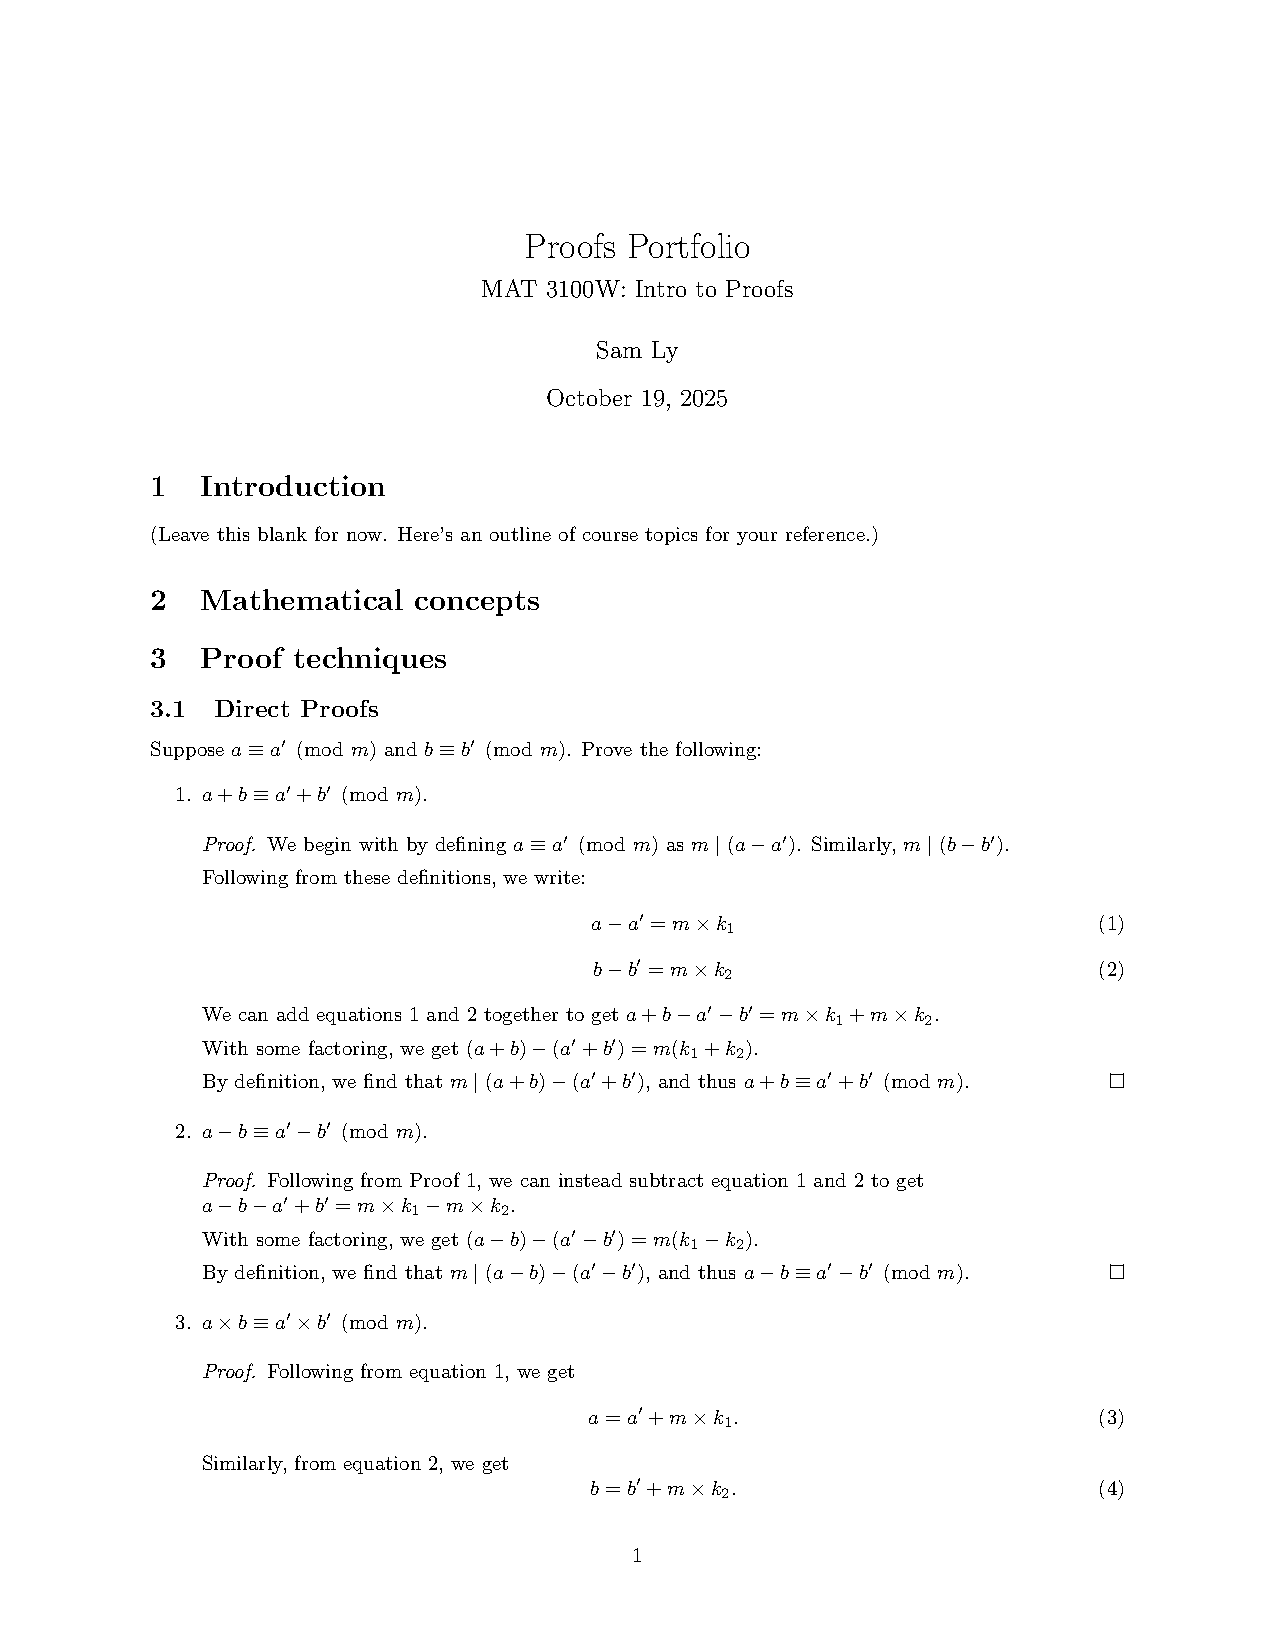
\includepdf[pages=-]{portfolio.pdf}
\end{document}